\documentclass[12pt]{article}
\usepackage[letterpaper]{geometry}
\usepackage{enumitem}
\usepackage[english]{babel}
\usepackage{graphicx}
\usepackage{tgcursor}
\usepackage[T1]{fontenc}

\setlength{\parindent}{0.0in}
%\setlength{\parskip}{1em}

%\renewcommand{\ttdefault}{pcr}

\setlist[itemize]{nosep}

\newcommand{\code}[1]{\texttt{#1}}

\title{PropXdoesWHAT}
\author{Chris Renard \and Dustin Huang \and Eder Garza \and Jae Lee \and Kevin Kuney}
\date{} % empty or it'll auto-pop with \today

\begin{document}

\maketitle

\section{Motivation}

We want to help users become aware of laws that affect them personally, particularly those in traditionally underrepresented groups. 
Since many laws can have complex side effects, due to both complexity in their primary purpose and the unfortunately common practice of including unrelated changes as riders, it can be difficult to keep up with legislation being worked on or voted on that could affect your life.
Marginalized groups especially can find changes that affect programs they may rely on buried in otherwise innocuous laws, or be unsure of what groups may be able to advocate for them or help them navigate changes.
Our goal is to allow groups to see what recent and upcoming laws may affect them and from there find groups which can better inform them and provide routes to take action against those which would harm them.


\section{User Stories}

The following are the user stories gathered for Phase 1: \\

\begin{itemize}
	\item\textbf{As a user, I want to be able to identify which groups are affected by a law.} \\
	We solved this issue by mapping the laws to the affected group and displaying them within each law model. In our API model, we set up a relationship between the laws and the affected groups. From there, we were able to call our API and display the mappings in a well-structured format using Bootstrap and ReactJS.
	\\
	
	\item\textbf{As a user, I want to see what congressmen, senators, city-council, etc. are supporting a law.} \\
	We solved this issue by mapping the laws to the corresponding politician and displaying them within each law model. In our API model, we set up a relationship between the laws and the policitians involved. From there, we were able to call our API and display the mappings in a well-structured format using Bootstrap and ReactJS.
	\\
	
	\item\textbf{As a user, I want to see where the politicians lie on the political spectrum.} \\
	We solved this issue by grabbing the politician's political affiliation from our API database and structuring the information using Bootstrap and ReactJS.
	\\
	
	\item\textbf{As a user, I want to see the implications of a law.} \\
	We solved this issue by having a description for each law. This was done by querying the description parameter data from our law API and displaying it onto the appropriate model page. 
	\\
	
	\item\textbf{As a user, I want to know how I can contact my senator/representative.} \\
	We solved this issue by displaying each politician's bio, which includes their website and number. This was done by querying the relevant contact information parameters from our API and displaying it onto our website with front-end tools, such as Bootstrap and ReactJS.
	
\end{itemize} ~\\


The following are the user stories gathered for Phase 2: \\
	
\begin{itemize}
	\item\textbf{As a user, I would like to see information about what the website does on the homepage.} \\
	We solved this issue by displaying the purpose of the website in the homepage.
	\\
	
	\item\textbf{As a user, I would like to see more laws, politicians associated with these laws, action groups, and affected groups.} \\
	We resolved this user story by having the front-end gather the data from the API and displaying it. Our models are linked with foreign keys creating relationships with each other. Within our JavaScript code, we displayed the necessary data which now displays more laws, politicians associated with these laws, action groups, and affected groups.
	\\
	
	\item\textbf{As a user, I would like each image on the front page carousel to lead me to a certain page.} \\
	We solved this issue by making each image a link to different pages.
	\\
	
	\item\textbf{As a user, I would like an easy way to contact a certain action group.} \\
	We solved this issue by displaying the necessary contact information of a certain action group on the model page. This was done through querying the data from our API and displaying it to the website with front-end tools such as Bootstrap and ReactJS.
	\\ 
	
	\item\textbf{As a user, I would like the affected group's website pages to have a little more info (do a little more than just list laws affecting group and action groups associated)} \\
	We solved this issue by displaying more than just laws and action groups related to this affected group. From our API model for affected groups, we queried the data and displayed it to the model web page for affected groups with front-end tools such as Bootstrap and ReactJS.
\end{itemize}

\section{Models}
    Each politician model shows each law and action group associated with them. Each law shows each politician and action group associated with them. Each affected group shows each politician and law associated with them. These associations lead to their respective model page. Each action group shows each law that affects the group. \\

\begin{itemize}
	\item[] Laws
	\begin{itemize}
		\item Name
		\item Title
		\item Description
		\item Sponsor
		\item Affected Groups (incoming table relation) (not built)
		\item Primary Subject
		\item Congress.gov Link
		\item GovTrack Link
		\item Date Introduced
		\item Date of last vote  (if occurred)
		\item Date bill passed Senate (if occurred)
		\item Date bill passed House (if occurred)
		\item Date bill was vetoed (if occurred)
		\item Date bill was enacted  (if occurred)
	\end{itemize}
	\item[] Politicians
	\begin{itemize}
		\item First Name
		\item Last Name
		\item State
		\item Party Affiliation
		\item Chamber (House or Senate)
		\item Phone
		\item Link to official site
		\item Link to contact page (if present)
	\end{itemize}
	\item[] Affected Groups
	\begin{itemize}
		\item Name
		\item Description
	\end{itemize}
	\item[] Action Groups
	\begin{itemize}
		\item Name
		\item Description
		\item Type/Category
		\item Link to official site
		\item Assisted groups (incoming table relation) (not built)
		\item Statements on laws (incoming table relation, text) (not built)
	\end{itemize}
\end{itemize}

\section{RESTful API}

API Endpoints: \\

\begin{itemize}
	\item api.propxdoeswhat.me/api/politicians
	\item api.propxdoeswhat.me/api/affected\_groups
	\item api.propxdoeswhat.me/api/action\_groups
	\item api.propxdoeswhat.me/api/laws
\end{itemize}

~\\
Full API Documentation at: documenter.getpostman.com/view/4704075/RWEmKHJp

\section{Tools}

\begin{itemize}
	\item Git		--- Version Control
	\item GitLab	--- Git repository hosting, issue tracking
	\item Postman	--- API design and testing % thing is a PoS though
	\item Grammarly	--- Spelling/grammar feedback for this report
	\item Piazza	--- Collecting User Stories from end users
	\item Slack		--- Team communication and collaboration
	\item Flask     --- 
	\item React     ---
	\item AWS       --- Server
\end{itemize}

\section{Setup}

\textbf{HOW WE SETUP TOOLS}

\section{Hosting}

\subsection{Database}

Our database is hosted on Amazon's Relational Database service. We used MySQL to design and populate our database.

\subsection{Back End}

The back end is hosted on an AWS EC2 instance. The main file is "Back-end/app.py" and it is running in a docker container on the server. The back end utilizes flask, sqlalchemy and flask-restless to create an API. The API is hosted on "api.propxdoeswhat.me/api/".

\subsection{Front End}

The front end is also hosted on an AWS EC2 instance. The main file is "Front-end/app.py" and it is running in a docker container on the server. We used React and Bootstap to build the front end. The front end gets data from our back end and serves it to the client. The front end is hosted on "propxdoeswhat.me".

\section{AWS}

First, we launched an EC2 instance with Amazon Linux AMI(Amazon Machine Image). Since by default, all incoming ports are blocked, we added security group rules that allow incoming SSH and HTTP requests from anywhere. Next, we SSH'd into the EC2 instance by using the private key file we were given as we launched the instance, the username EC2-user, and the public IP address of the instance. \\

Frontend access: \\
\code{ssh -i front-end-private-key.pem ec2-user@propxdoeswhat.me} \\
Backend access: \\
\code{ssh -i back-end-private-key.pem ec2-user@api.propxdoeswhat.me} \\

Next, we updated the working Linux server running in the AWS cloud and installed docker on it. Then, we transferred our local files onto the server using FileZilla's SSH File Transfer Protocol. Finally, we built our Docker image and ran our web application on our Docker container.

\section{Database}

We use a MySQL 5.6 instance running on Amazon RDS. The Amazon default settings use \code{latin1} for text (this is bad), we had to manually adjust them to use \code{utf8mb4} and rebuild tables. Note: \code{utf8} in MySQL does not meet the utf8 spec, as it will not work with astral glyphs (four-byte characters). While this is unlikely to occur in our dataset, for future-proofing we use \code{utf8mb4} which correctly implements the standard. 

\begin{itemize}
	\item[] `laws`
	\begin{itemize}
		\item \code{`id` INT UNSIGNED NOT NULL AUTO\_INCREMENT}	-- internal id, auto-generated
		\item \code{`bill\_id` VARCHAR(32) NOT NULL}			-- unique bill name across legislatures, ie: hr5515-115
		\item \code{`name` VARCHAR(32) NOT NULL}				-- name of bill, ie: H.R.5515
		\item \code{`title` VARCHAR(256) NOT NULL}				-- short title of bill
		\item \code{`subject` VARCHAR(256) NOT NULL}			-- primary subject of bill
		\item \code{`sponsor\_id` INT UNSIGNED NOT NULL}		-- foreign key to `politicians`
		\item \code{`sponsor\_bio\_id` VARCHAR(16) NOT NULL}	-- Biography of Congress unique id for sponsor, ie: T000238
		\item \code{`cdotgov\_url` VARCHAR(256),}				-- url of bill on congress.gov
		\item \code{`govtrack\_url` VARCHAR(256),}				-- url of bill on govtrack
		\item \code{`introduced` DATE}
		\item \code{`last\_vote` DATE}
		\item \code{`house\_pass` DATE}
		\item \code{`senate\_pass` DATE}
		\item \code{`enacted` DATE}
		\item \code{`vetoed` DATE}
		\item \code{`desc` TEXT}								-- propublica summary
		\item \code{`raw` TEXT}									-- raw json from source for this entry
	\end{itemize}
	\item[] Politicians
	\begin{itemize}
		\item \code{`id` INT UNSIGNED NOT NULL AUTO\_INCREMENT}	-- internal id, auto-generated
		\item \code{`first\_name` VARCHAR(64) NOT NULL}
		\item \code{`last\_name` VARCHAR(64) NOT NULL}
		\item \code{`dob` DATE NOT NULL}						-- date of birth
		\item \code{`bio\_id` VARCHAR(16) NOT NULL}				-- Biography of Congress unique id, ie: T000238
		\item \code{`chamber` ENUM('house', 'senate') NOT NULL}
		\item \code{`state` CHAR(2) NOT NULL}
		\item \code{`party` ENUM('R', 'D', 'I') NOT NULL}
		\item \code{`site` VARCHAR(256)}						-- url for official site
		\item \code{`contact\_form` VARCHAR(256)}				-- url for official contact form
		\item \code{`phone` VARCHAR(32)}
		\item \code{`raw` TEXT}									-- raw json from source for this entry
	\end{itemize}
	\item[] Action Groups
	\begin{itemize}
		\item \code{`id` INT UNSIGNED NOT NULL AUTO\_INCREMENT}	-- internal id, auto-generated
		\item \code{`name` VARCHAR(256) NOT NULL}
		\item \code{`url` VARCHAR(256) NOT NULL}				-- url of official site
		\item \code{`type` VARCHAR(256) NOT NULL}				-- startguide.org category of group
		\item \code{`desc` TEXT}
	\end{itemize}
\end{itemize}

%\begin{figure}[h!]
%  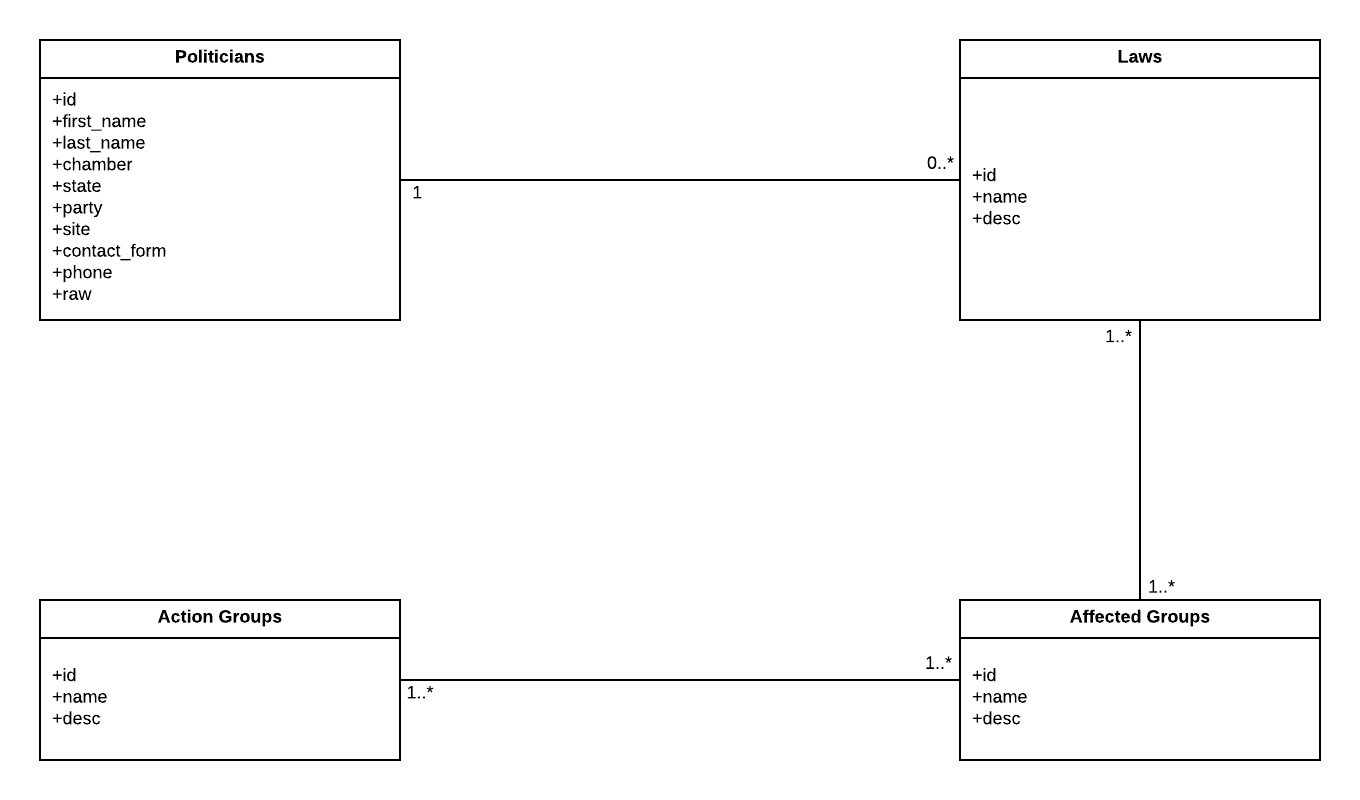
\includegraphics[width=\linewidth]{../Group8_UML.png}
%\end{figure}

\section{Pagination}

For our models, the data in our database contains a large number of instances of laws, politicians, action groups, and affected groups. To give the user a better experience navigating through all of our data, we implemented a traditional pagination number system. Our API paginates all the data. Using React components and Bootstrap, we created functionality to the buttons. Our pagination number system contains a previous page, next page, page items, and a page footer.

\section{Testing}



\end{document}